%!tex program = lualatex
\documentclass{ctexart}
\usepackage{amsmath, amssymb}
\usepackage{xcolor}
\ctexset{
  section/name = {问题},
  section/nameformat += {\sffamily},
  section/numberformat += {\color{magenta}\Huge}
}
%%%%%%%%%%%%%%%%%%%%%%%%%%%%%%%%%%%%%%%%%%%%%%%%%%%%%%%%%%%%%%%%%%%%%%%%%%%%%%%
\usepackage[most]{tcolorbox}
\usetikzlibrary{arrows.meta}
%%%%%%%%%%%%%%%%%%%%%%%%%%%%%%%%%%%%%%%%%%%%%%%%%%%%%%%%%%%%%%%%%%%%%%%%%%%%%%%
\usepackage{algorithm}
\usepackage{algpseudocodex}
\usepackage{caption}
\captionsetup[algorithm]{name={算法}}
%%%%%%%%%%%%%%%%%%%%%%%%%%%%%%%%%%%%%%%%%%%%%%%%%%%%%%%%%%%%%%%%%%%%%%%%%%%%%%%
\usepackage{silence}
\WarningFilter{latexfont}{Font shape}
\WarningFilter{latexfont}{Size substitutions}
\WarningFilter{latexfont}{Some font}
\hfuzz=15pt
%%%%%%%%%%%%%%%%%%%%%%%%%%%%%%%%%%%%%%%%%%%%%%%%%%%%%%%%%%%%%%%%%%%%%%%%%%%%%%%
\usepackage{hyperref}
\hypersetup{
  colorlinks = true,
  urlcolor = magenta,
  linkcolor = cyan
}
\begin{document}
\chapter{Multiples of 3 or 5}
\section{Description}
If we list all the natural numbers below 10 that are multiples of 3 or 5, we get 3, 5, 6 and 9. The sum of these multiples is 23.

Find the sum of all the multiples of 3 or 5 below 1000.
试试看中文能不能显示?
\section{Flow Chart}

\begin{center}
	\begin{tikzpicture}[node distance=2cm]
		\node (start) [startstop] {开始};
		\node (in1) [io, right of=start, xshift=3cm] {输入一个上限cap};
		\node (pro1) [operation, right of=in1, xshift=3cm] {n = 1\\
			sum = 0};
		\node (dec1) [decision, below of=pro1, yshift=-1cm] {n能被3\\
			或者5整除};
		\node (pro2) [yshift=-1cm, operation, below of = dec1] {sum += n;\\
			++n;};
		\node (dec2) [decision, below of=pro2, yshift=-.5cm] {n < cap};
		\node (out1) [io, left of=dec2, xshift=-3cm] {输出数据};
		\node (stop) [startstop, left of=out1, xshift=-3cm] {终止};

		\draw [arrow] (start) -- (in1);
		\draw [arrow] (in1) -- (pro1);
		\draw [arrow] (pro1) -- (dec1);
		\draw [arrow] (dec1) -- node[anchor=east] {Yes}(pro2);
		\draw [arrow] (pro2) --  (dec2);
		\draw [arrow] (dec2.west) -- node[above] {No} (out1);
		\draw [arrow] (dec2.east) -| ([xshift=2cm]dec1.east) -- node[anchor=south east, text centered] {Yes} (dec1.east);
		\draw [arrow] (out1) -- (stop);
	\end{tikzpicture}
	\captionof{figure}{Multiples of 3 or 5}
\end{center}

\section{Codes}
\begin{cpp}
	long Solution::sum_of_multiples(int cap)
	{
			long sum{};

			for(int i{1}; i < cap; ++i)
			{
					if(i % 3 == 0 || i % 5 == 0) sum += i;
				}
			return sum;
		}
\end{cpp}

\section{title}
\subsection{Problem Description}
\begin{tcolorbox}

\end{tcolorbox}
		

\section{title}
\subsection{Problem Description}
\begin{tcolorbox}

\end{tcolorbox}
		

\section{title}
\subsection{Problem Description}
\begin{tcolorbox}

\end{tcolorbox}
		

\section{最小公倍数}\label{sec:problem05}
\subsection{问题描述}
\begin{tcolorbox}
	2520 是能够被 1 到 10 的每个数字整除的最小数字。

	求最小的正整数,使得它能够被 1 到 20 的每个数字整除。
\end{tcolorbox}

\subsection{算法}
最大公约数在STL中有提供,但是做为数学及编程的最基本的内容,还是有必要自己写一下的。

\textbf{数学原理}:

欧几里得算法基于这样一个定理:两个整数  $ a $  和  $ b $  的最大公约数等于  $b$  和 \( a \mod b \) 的最大公约数,其中 \(
a \mod b \) 是  $a$  除以  $b$  的余数。

\begin{algorithm}
	\caption{最大公约数}
	\begin{algorithmic}[1]
		\Function{Gcd}{$a, b$}
		\While{b \neq 0}
		\State $ temp = a$
		\State $ a = b$
		\State $ b = temp \mod b$
		\EndWhile
		\Return $a$
		\EndFunction
	\end{algorithmic}
\end{algorithm}

\begin{algorithm}
	\caption{最小公倍数}
	\begin{algorithmic}[1]
		\Function{Lcm}{$a, b$}
			\If{$a = 0 \text{ or } b = 0$}
				\Return $0$
			\EndIf
			\Return $\left|\frac{a \times b}{\text{gcd}(a,b)}\right|$
		\EndFunction
	\end{algorithmic}
\end{algorithm}

\subsection{答案}
232792560

\section{平方和之差}
\subsection{问题描述}
\begin{tcolorbox}
	前十个自然数的平方和是:

	\[
		1^2 + 2^2 + \dots + 10^2 = 385
	\]

	前十个自然数的和的平方是:

	\[
		(1 + 2 + \dots + 10)^2 = 55^2 = 3025
	\]

	因此,和的平方与平方和之间的差为 \( 3025 - 385 = 2640 \)。

	请找到前 100 个自然数的和的平方与平方和之间的差。
\end{tcolorbox}

\subsection{答案}
 25164150

\section{第10001个质数}
\subsection{问题描述}
\begin{tcolorbox}
通过列出前六个质数:2, 3, 5, 7, 11 和 13,可以看到第六个质数是 13。

求第 10001 个质数是多少?
\end{tcolorbox}

\subsection{算法}

\subsection{答案}

\section{数列中的最大乘积}\label{sec:problem08}
\subsection{问题描述}
\begin{tcolorbox}
在下面这个 1000 位的数字中,相邻的四个数字的最大乘积是 9 × 9 × 8 × 9 = 5832。

\begin{verbatim}
73167176531330624919225119674426574742355349194934
96983520312774506326239578318016984801869478851843
85861560789112949495459501737958331952853208805511
12540698747158523863050715693290963295227443043557
66896648950445244523161731856403098711121722383113
62229893423380308135336276614282806444486645238749
30358907296290491560440772390713810515859307960866
70172427121883998797908792274921901699720888093776
65727333001053367881220235421809751254540594752243
52584907711670556013604839586446706324415722155397
53697817977846174064955149290862569321978468622482
83972241375657056057490261407972968652414535100474
82166370484403199890008895243450658541227588666881
16427171479924442928230863465674813919123162824586
17866458359124566529476545682848912883142607690042
24219022671055626321111109370544217506941658960408
07198403850962455444362981230987879927244284909188
84580156166097919133875499200524063689912560717606
05886116467109405077541002256983155200055935729725
71636269561882670428252483600823257530420752963450
\end{verbatim}

找出这个 1000 位数字中,相邻的 13 个数字的乘积最大的值。这个最大的乘积是多少?
\end{tcolorbox}

\subsection{算法}
这道题比较简单,只要遍历即可。如果遇到0就直接跳到0后面的数字再开始。

需要注意的是这个算法中会用字符串来表示大数字,所以取出的数字是字符,需要做相应的运算才能成为数值。

\subsection{答案}
23514624000

\section{特殊勾股数}\label{sec:problem09}
\subsection{问题描述}
\begin{tcolorbox}
	一组勾股数是一组三个自然数 \( a < b < c \),使得:

	\[
		a^2 + b^2 = c^2
	\]

	例如,\( 3^2 + 4^2 = 9 + 16 = 25 = 5^2 \)。

	有且只有一组勾股数满足 \( a + b + c = 1000 \)。求出这组勾股数中 \( abc \) 的乘积。
\end{tcolorbox}

\subsection{算法}
这道题只需要遍历即可实现求解,值得考虑的地方是遍历的边界。因为三角形的一条边肯定小于另外两条边的和(勾股数可以看作直角三角形的三条边),所以斜边
\( c \) 最多不会超过499,而 \( a + b + c = 0, c > a, c > b \), 所以有 \( c \geqslant 334 \)。

\subsection{答案}
31875000

\section{质数之和}\label{sec:problem10}
\subsection{问题描述}
\begin{tcolorbox}
小于 10 的质数的和是 \(2 + 3 + 5 + 7 = 17\)。

请找出所有小于两百万的质数的和。
\end{tcolorbox}

\subsection{算法}
用问题\ref{sec:prime}中的筛法即可解决。

\subsection{答案}
142913828922

\section{矩阵中的最大乘积}
\subsection{问题描述}
\begin{tcolorbox}
	在下面这个 20×20 的网格中,沿对角线的四个相邻数字已经标记为红色,这些数字的乘积是 \(  26 \times 63 \times 78 \times 14 = 1788696 \) 。
	\begin{equation*}
		\begin{array}{@{\hspace{4pt}}c@{\hspace{4pt}}c@{\hspace{4pt}}c@{\hspace{4pt}}c@{\hspace{4pt}}c@{\hspace{4pt}}c@{\hspace{4pt}}c@{\hspace{4pt}}c@{\hspace{4pt}}c@{\hspace{4pt}}c@{\hspace{4pt}}c@{\hspace{4pt}}c@{\hspace{4pt}}c@{\hspace{4pt}}c@{\hspace{4pt}}c@{\hspace{4pt}}c@{\hspace{4pt}}c@{\hspace{4pt}}c@{\hspace{4pt}}c@{\hspace{4pt}}c}
			08 & 02 & 22 & 97 & 38 & 15 & 00 & 40 & 00                  & 75                  & 04                  & 05                  & 07 & 78 & 52 & 12 & 50 & 77 & 91 & 08 \\
			49 & 49 & 99 & 40 & 17 & 81 & 18 & 57 & 60                  & 87                  & 17                  & 40                  & 98 & 43 & 69 & 48 & 04 & 56 & 62 & 00 \\
			81 & 49 & 31 & 73 & 55 & 79 & 14 & 29 & 93                  & 71                  & 40                  & 67                  & 53 & 88 & 30 & 03 & 49 & 13 & 36 & 65 \\
			52 & 70 & 95 & 23 & 04 & 60 & 11 & 42 & 69                  & 24                  & 68                  & 56                  & 01 & 32 & 56 & 71 & 37 & 02 & 36 & 91 \\
			22 & 31 & 16 & 71 & 51 & 67 & 63 & 89 & 41                  & 92                  & 36                  & 54                  & 22 & 40 & 40 & 28 & 66 & 33 & 13 & 80 \\
			24 & 47 & 32 & 60 & 99 & 03 & 45 & 02 & 44                  & 75                  & 33                  & 53                  & 78 & 36 & 84 & 20 & 35 & 17 & 12 & 50 \\
			32 & 98 & 81 & 28 & 64 & 23 & 67 & 10 & \textcolor{red}{26} & 38                  & 40                  & 67                  & 59 & 54 & 70 & 66 & 18 & 38 & 64 & 70 \\
			67 & 26 & 20 & 68 & 02 & 62 & 12 & 20 & 95                  & \textcolor{red}{63} & 94                  & 39                  & 63 & 08 & 40 & 91 & 66 & 49 & 94 & 21 \\
			24 & 55 & 58 & 05 & 66 & 73 & 99 & 26 & 97                  & 17                  & \textcolor{red}{78} & 78                  & 96 & 83 & 14 & 88 & 34 & 89 & 63 & 72 \\
			21 & 36 & 23 & 09 & 75 & 00 & 76 & 44 & 20                  & 45                  & 35                  & \textcolor{red}{14} & 00 & 61 & 33 & 97 & 34 & 31 & 33 & 95 \\
			78 & 17 & 53 & 28 & 22 & 75 & 31 & 67 & 15                  & 94                  & 03                  & 80                  & 04 & 62 & 16 & 14 & 09 & 53 & 56 & 92 \\
			16 & 39 & 05 & 42 & 96 & 35 & 31 & 47 & 55                  & 58                  & 88                  & 24                  & 00 & 17 & 54 & 24 & 36 & 29 & 85 & 57 \\
			86 & 56 & 00 & 48 & 35 & 71 & 89 & 07 & 05                  & 44                  & 44                  & 37                  & 44 & 60 & 21 & 58 & 51 & 54 & 17 & 58 \\
			19 & 80 & 81 & 68 & 05 & 94 & 47 & 69 & 28                  & 73                  & 92                  & 13                  & 86 & 52 & 17 & 77 & 04 & 89 & 55 & 40 \\
			04 & 52 & 08 & 83 & 97 & 35 & 99 & 16 & 07                  & 97                  & 57                  & 32                  & 16 & 26 & 26 & 79 & 33 & 27 & 98 & 66 \\
			88 & 36 & 68 & 87 & 57 & 62 & 20 & 72 & 03                  & 46                  & 33                  & 67                  & 46 & 55 & 12 & 32 & 63 & 93 & 53 & 69 \\
			04 & 42 & 16 & 73 & 38 & 25 & 39 & 11 & 24                  & 94                  & 72                  & 18                  & 08 & 46 & 29 & 32 & 40 & 62 & 76 & 36 \\
			20 & 69 & 36 & 41 & 72 & 30 & 23 & 88 & 34                  & 62                  & 99                  & 69                  & 82 & 67 & 59 & 85 & 74 & 04 & 36 & 16 \\
			20 & 73 & 35 & 29 & 78 & 31 & 90 & 01 & 74                  & 31                  & 49                  & 71                  & 48 & 86 & 81 & 16 & 23 & 57 & 05 & 54 \\
			01 & 70 & 54 & 71 & 83 & 51 & 54 & 69 & 16                  & 92                  & 33                  & 48                  & 61 & 43 & 52 & 01 & 89 & 19 & 67 & 48
		\end{array}
	\end{equation*}
相邻(上下左右对角线)的四个数字乘积的最大值是多少?
\end{tcolorbox}

\subsection{算法}
遍历,注意边界。另外,也要考虑反对角线。

\subsection{答案}
70600674

\section{高度可被整除的三角形数}\label{sec:problem12}
\subsection{问题描述}
\begin{tcolorbox}
	三角形数序列是通过逐个加上自然数来生成的。也就是说,第七个三角形数是

	\[
		1 + 2 + 3 + 4 + 5 + 6 + 7 = 28
	\]

	前十个三角形数是:

	\[
		1, 3, 6, 10, 15, 21, 28, 36, 45, 55, \ldots
	\]


	前七个三角形数的约数为:
	\begin{align*}
		\mathbf 1   & \colon 1             \\
		\mathbf 3   & \colon 1,3           \\
		\mathbf 6   & \colon 1,2,3,6       \\
		\mathbf{10} & \colon 1,2,5,10      \\
		\mathbf{15} & \colon 1,3,5,15      \\
		\mathbf{21} & \colon 1,3,7,21      \\
		\mathbf{28} & \colon 1,2,4,7,14,28
	\end{align*}
	我们可以看到,28 的约数有:1, 2, 4, 7, 14, 28。
	第一个拥有超过五个约数的三角形数是 28。

	第一个拥有超过 500 个约数的三角形数是多少?
\end{tcolorbox}

\subsection{算法}
\begin{algorithm}[H]
	\caption{算法标题}
	\begin{algorithmic}[1]
	\Function{CountDivisors}{$N$}
	\State $root \gets \lfloor \sqrt{N} \rfloor$
	\State $ count \gets 0$
	\For{$i \gets 1$ to $root$}
	\State $count \gets count + 2$
	\EndFor
	\If{$root \times root = N$}
	\State $count \gets count - 1$
	\EndIf
	\Return $count$
	\EndFunction
	\end{algorithmic}
\end{algorithm}

\subsection{答案}
76576500

\section{大数加法}
\subsection{问题描述}
\begin{tcolorbox}[breakable]
下列是一百个 50 位的数字:

\begin{center}
37107287533902102798797998220837590246510135740250 \\
46376937677490009712648124896970078050417018260538 \\
74324986199524741059474233309513058123726617309629 \\
91942213363574161572522430563301811072406154908250 \\
23067588207539346171171980310421047513778063246676 \\
89261670696623633820136378418383684178734361726757 \\
28112879812849979408065481931592621691275889832738 \\
44274228917432520321923589422876796487670272189318 \\
47451445736001306439091167216856844588711603153276 \\
70386486105843025439939619828917593665686757934951 \\
62176457141856560629502157223196586755079324193331 \\
64906352462741904929101432445813822663347944758178 \\
92575867718337217661963751590579239728245598838407 \\
58203565325359399008402633568948830189458628227828 \\
80181199384826282014278194139940567587151170094390 \\
35398664372827112653829987240784473053190104293586 \\
86515506006295864861532075273371959191420517255829 \\
71693888707715466499115593487603532921714970056938 \\
54370070576826684624621495650076471787294438377604 \\
53282654108756828443191190634694037855217779295145 \\
36123272525000296071075082563815656710885258350721 \\
45876576172410976447339110607218265236877223636045 \\
17423706905851860660448207621209813287860733969412 \\
81142660418086830619328460811191061556940512689692 \\
51934325451728388641918047049293215058642563049483 \\
62467221648435076201727918039944693004732956340691 \\
15732444386908125794514089057706229429197107928209 \\
55037687525678773091862540744969844508330393682126 \\
18336384825330154686196124348767681297534375946515 \\
80386287592878490201521685554828717201219257766954 \\
78182833757993103614740356856449095527097864797581 \\
16726320100436897842553539920931837441497806860984 \\
48403098129077791799088218795327364475675590848030 \\
87086987551392711854517078544161852424320693150332 \\
59959406895756536782107074926966537676326235447210 \\
69793950679652694742597709739166693763042633987085 \\
41052684708299085211399427365734116182760315001271 \\
65378607361501080857009149939512557028198746004375 \\
35829035317434717326932123578154982629742552737307 \\
94953759765105305946966067683156574377167401875275 \\
88902802571733229619176668713819931811048770190271 \\
25267680276078003013678680992525463401061632866526 \\
36270218540497705585629946580636237993140746255962 \\
24074486908231174977792365466257246923322810917141 \\
91430288197103288597806669760892938638285025333403 \\
34413065578016127815921815005561868836468420090470 \\
23053081172816430487623791969842487255036638784583 \\
11487696932154902810424020138335124462181441773470 \\
63783299490636259666498587618221225225512486764533 \\
67720186971698544312419572409913959008952310058822 \\
95548255300263520781532296796249481641953868218774 \\
76085327132285723110424803456124867697064507995236 \\
37774242535411291684276865538926205024910326572967 \\
23701913275725675285653248258265463092207058596522 \\
29798860272258331913126375147341994889534765745501 \\
18495701454879288984856827726077713721403798879715 \\
38298203783031473527721580348144513491373226651381 \\
34829543829199918180278916522431027392251122869539 \\
40957953066405232632538044100059654939159879593635 \\
29746152185502371307642255121183693803580388584903 \\
41698116222072977186158236678424689157993532961922 \\
62467957194401269043877107275048102390895523597457 \\
23189706772547915061505504953922979530901129967519 \\
86188088225875314529584099251203829009407770775672 \\
11306739708304724483816533873502340845647058077308 \\
82959174767140363198008187129011875491310547126581 \\
97623331044818386269515456334926366572897563400500 \\
42846280183517070527831839425882145521227251250327 \\
55121603546981200581762165212827652751691296897789 \\
32238195734329339946437501907836945765883352399886 \\
75506164965184775180738168837861091527357929701337 \\
62177842752192623401942399639168044983993173312731 \\
32924185707147349566916674687634660915035914677504 \\
99518671430235219628894890102423325116913619626622 \\
73267460800591547471830798392868535206946944540724 \\
76841822524674417161514036427982273348055556214818 \\
97142617910342598647204516893989422179826088076852 \\
87783646182799346313767754307809363333018982642090 \\
10848802521674670883215120185883543223812876952786 \\
71329612474782464538636993009049310363619763878039 \\
62184073572399794223406235393808339651327408011116 \\
66627891981488087797941876876144230030984490851411 \\
60661826293682836764744779239180335110989069790714 \\
85786944089552990653640447425576083659976645795096 \\
66024396409905389607120198219976047599490197230297 \\
64913982680032973156037120041377903785566085089252 \\
16730939319872750275468906903707539413042652315011 \\
94809377245048795150954100921645863754710598436791 \\
78639167021187492431995700641917969777599028300699 \\
15368713711936614952811305876380278410754449733078 \\
40789923115535562561142322423255033685442488917353 \\
44889911501440648020369068063960672322193204149535 \\
41503128880339536053299340368006977710650566631954 \\
81234880673210146739058568557934581403627822703280 \\
82616570773948327592232845941706525094512325230608 \\
22918802058777319719839450180888072429661980811197 \\
77158542502016545090413245809786882778948721859617 \\
72107838435069186155435662884062257473692284509516 \\
20849603980134001723930671666823555245252804609722 \\
53503534226472524250874054075591789781264330331690 \\
\end{center}

这些数字的总和为多少?请只给出前十位数字。
\end{tcolorbox}

\subsection{算法}
这道题需要实现字符串数字的加法,为了以后方面,可以设计一个字符串数字的类。当然也可以借鉴Python中无限大整数的实现方式。

\subsection{答案}
5537376230

\section{最长考拉兹序列}
\subsection{问题描述}
\begin{tcolorbox}
考拉兹序列是这样定义的:

\begin{itemize}
    \item 对于任意正整数 $n$,如果 $n$ 是偶数,则下一项是 $n / 2$;
    \item 如果 $n$ 是奇数,则下一项是 $3n + 1$。
\end{itemize}

使用这个规则不断重复,最终序列会到达 1。例如,使用 13 生成的考拉兹序列如下:

\[
13 \to 40 \to 20 \to 10 \to 5 \to 16 \to 8 \to 4 \to 2 \to 1
\]

这个序列有 10 项。尽管尚未被证明(称为考拉兹猜想),但相信所有的起始数字最终都能到达 1。

哪一个起始数字,$n < 1,000,000$,能够生成最长的序列?
\end{tcolorbox}

\subsection{算法}
这道题只需要遍历即可。

\subsection{答案}

\section{格子路径}\label{sec:problem15}
\subsection{网格中的路径}
\begin{tcolorbox}
	从一个 $2 \times 2$网格的左上角出发,只能向下与向右移动,到达有理解一共有6条路径。

	\begin{center}
		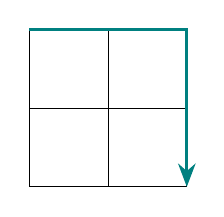
\begin{tikzpicture}
			\draw (0, 0) grid +(2,2);
			\draw[very thick, -Stealth, blue!50!green] (0, 2) -| (2, 0);
		\end{tikzpicture}
		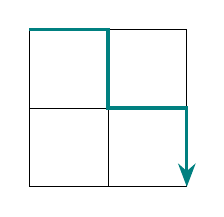
\begin{tikzpicture}
			\draw (0, 0) grid +(2,2);
			\draw[very thick, -Stealth, blue!50!green] (0, 2) -| (1, 1) -| (2,0);
		\end{tikzpicture}
		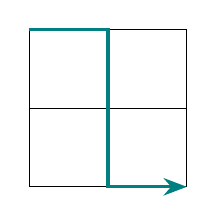
\begin{tikzpicture}
			\draw (0, 0) grid +(2,2);
			\draw[very thick, -Stealth, blue!50!green] (0, 2) -| (1, 0) -- (2, 0);
		\end{tikzpicture}

		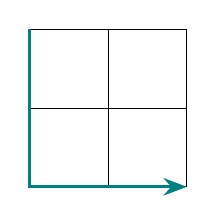
\begin{tikzpicture}
			\draw (0, 0) grid +(2,2);
			\draw[very thick, -Stealth, blue!50!green] (0, 2) |- (2, 0);
		\end{tikzpicture}
		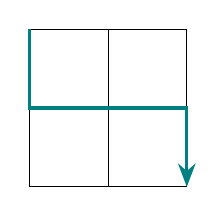
\begin{tikzpicture}
			\draw (0, 0) grid +(2,2);
			\draw[very thick, -Stealth, blue!50!green] (0, 2) |- (1, 1) -| (2,0);
		\end{tikzpicture}
		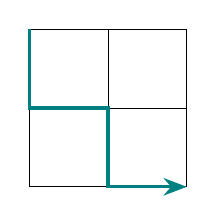
\begin{tikzpicture}
			\draw (0, 0) grid +(2,2);
			\draw[very thick, -Stealth, blue!50!green] (0, 2) |- (1, 1) |- (2,0);
		\end{tikzpicture}
	\end{center}

	在一个 $20 \times 20$ 的网格中,从左上角到右下角的路径,每次只能向右或向下移动一次。有多少条不同的路径从起点到终点?
\end{tcolorbox}

\subsection{算法}
这道题目要用到动态规划来解,最上边的第一个节点都依赖于其左边的节点有多少路径,与最上边相似,最左边的节点都依赖其上面的节点,在这里最上边与最左边的节点的路径数都为1。其他节点都依赖于其上方与左边的节点的数量,因此可以写成下面的伪代码:
\begin{algorithm}
	\caption{网格路径数}
	\begin{algorithmic}[1]
	\State 初始化一个 $(N+1) \times (N+1)$的矩阵,第1行全部为1,第一列也全部为1
	\State 遍历除第一行和第一列以外的节点,每个节点的值等于上方的值+左边的值
	\end{algorithmic}
\end{algorithm}


\subsection{答案}
137846528820

\section{数字的数字和}
\subsection{问题描述}
\begin{tcolorbox}
2 的 15 次方是 32768,其数字和为 3 + 2 + 7 + 6 + 8 = 26。

计算 2 的 1000 次方的数字和是多少?
\end{tcolorbox}

\subsection{算法}
可以将字符串数字类中实现一个乘法,在乘法的基础上实现幂运算。然后还需要实现一个计算数字和的函数。

\subsection{答案}

\section{数字文字计数}
\subsection{问题描述}
\begin{tcolorbox}
	如果将 1 到 5 写成英文单词,它们分别是:

	\begin{itemize}
		\forcsvlist{\item}{
		      1 = "one",
		      2 = "two",
		      3 = "three",
		      4 = "four",
		      5 = "five",
		      }
	\end{itemize}
	这些单词的字母数量为 3、3、5、4 和 4。因此,1 到 5 的数字单词一共有
	$ 3 + 3 + 5 + 4 + 4 = 19 $
	个字母。

	从 1 到 1000(含 1000)中的每个数字用英文单词来表示,不计空格和连字符,总共有多少个字母?

	例如:
	342(three hundred and forty-two)包含 23 个字母。

	115(one hundred and fifteen)包含 20 个字母。

	注意:不计空格或连字符,"and" 是按规则包含在使用中的英文单词中。
\end{tcolorbox}

\subsection{算法}
\begin{enumerate}
	\item 准备数字到英文单词的映射表:我们需要将 1 到 19 的单词直接映射。对于整十数(20, 30, ..., 90),也要单独映射。然后为“hundred”(100)和“thousand”(1000)定义规则。
	\item 分段处理数字:例如,对于 342,英文单词表示为 \textit{three hundred and forty-two}。我们可以将数字拆分为百位数、十位数、个位数,分别进行转换。
	\item 处理特殊情况:例如 100 到 999 之间的数字,需要注意添加 "and"。
	\item 统计字母数:统计所有数字转换成单词后的字母数量,不计空格和连字符。
\end{enumerate}

\subsection{答案}
21124

\section{最大路径和}
\subsection{问题描述}
\begin{tcolorbox}
	给定一个三角形,从顶部到底部选择一条路径,使得路径上的数字总和最大。如下所示:

	\[
		\begin{aligned}
			  &   &                    & \textcolor{red}{3} &                    &   &   \\
			  &   & \textcolor{red}{7} &                    & 4                  &   &   \\
			  & 2 &                    & \textcolor{red}{4} &                    & 6 &   \\
			8 &   & 5                  &                    & \textcolor{red}{9} &   & 3
		\end{aligned}
	\]

	在这个例子中,最大的路径和为 23。请找到这个最大路径和。

	\begin{center}
		75\\
		95 64\\
		17 47 82\\
		18 35 87 10\\
		20 04 82 47 65\\
		19 01 23 75 03 34\\
		88 02 77 73 07 63 67\\
		99 65 04 28 06 16 70 92\\
		41 41 26 56 83 40 80 70 33\\
		41 48 72 33 47 32 37 16 94 29\\
		53 71 44 65 25 43 91 52 97 51 14\\
		70 11 33 28 77 73 17 78 39 68 17 57\\
		91 71 52 38 17 14 91 43 58 50 27 29 48\\
		63 66 04 68 89 53 67 30 73 16 69 87 40 31\\
		04 62 98 27 23 09 70 98 73 93 38 53 60 04 23\\
	\end{center}
\end{tcolorbox}

\subsection{算法}
这道题目用动态规划的方法来求解。

\subsection{答案}
1074

\section{标题}
\subsection{问题描述}
\begin{tcolorbox}
在1901年1月1日到2000年12月31日的这段时间内,有多少个月的1号是星期天?已知:
\begin{itemize}
    \item 1900年1月1日是星期一;
    \item 闰年规则为:如果年份能被4整除但不能被100整除,或者能被400整除,则该年为闰年;
    \item 每月天数:
    \begin{itemize}
        \item 31天:1月、3月、5月、7月、8月、10月、12月;
        \item 30天:4月、6月、9月、11月;
        \item 28天:2月,闰年为29天。
    \end{itemize}
\end{itemize}
\end{tcolorbox}

\subsection{算法}
先实现一个闰年判断的函数
\begin{algorithm}
	\caption{算法标题}
	\begin{algorithmic}[1]
		\If{$Y \mod 400 = 0$ or $(Y \mod 4 = 0$ and $Y \mod 100 \neq 0) $}
		\Return \textbf{true}
	\EndIf
	\end{algorithmic}
\end{algorithm}

\subsection{答案}

\section{阶乘数字和}
\subsection{问题描述}
\begin{tcolorbox}
求 $100!$ 的各位数字和。即:
\[
100! = 100 \times 99 \times \cdots \times 2 \times 1
\]
计算得到的阶乘结果后,求其各位数字的和。例如:
\[
10! = 10 \times 9 \times \cdots \times 1 = 3628800
\]
其各位数字之和为:
\[
3 + 6 + 2 + 8 + 8 + 0 + 0 = 27
\]
\end{tcolorbox}

\subsection{算法}
用前面实现的字符串数字类中添加个阶乘的算法。

\subsection{答案}
648

\section{亲和数之和}\label{sec:problem21}
\subsection{问题描述}
\begin{tcolorbox}
	定义 $d(n)$ 表示 $n$ 的所有真因数(即小于 $n$ 的除 $n$ 之外的除数)的和。

	如果 $d(a) = b$ 且 $d(b) = a$,并且 $a \neq b$,那么 $a$ 和 $b$ 被称为亲和数。例如,220 和 284 就是一对亲和数:

	\[
		d(220) = 1 + 2 + 4 + 5 + 10 + 11 + 20 + 22 + 44 + 55 + 110 = 284
	\]
	\[
		d(284) = 1 + 2 + 4 + 71 + 142 = 220
	\]

	求小于10000的所有亲和数的和。
\end{tcolorbox}

\subsection{算法}
\begin{enumerate}
	\item 编写函数 $d(n)$,计算 $n$ 的所有真因数的和。
	\item 对于每个小于10000的数字 $a$,计算 $b = d(a)$,如果 $d(b) = a$ 且 $a \neq b$,则 $a$ 和 $b$ 是亲和数。
	\item 注意避免重复计算。
\end{enumerate}

\subsection{答案}
31626

\section{名字记分}\label{sec:problem22}
\subsection{问题描述}
\begin{tcolorbox}

给定一个超过五千个名字的文件,将这些名字按字母顺序排序。然后,对于每个名字,按以下步骤计算得分:

\begin{enumerate}
    \item 计算名字的字母值:将名字中每个字母的字母顺序($A=1, B=2, ..., Z=26$)相加。例如,$COLIN$ 的字母值为 $3 + 15 + 12 + 9 + 14 = 53$。
    \item 将名字的字母值乘以其在排序后的位置索引,得到名字的得分。例如,"COLIN" 在排序后是第938个名字,其得分为 $938 \times 53 = 49714$。
\end{enumerate}
\end{tcolorbox}

\subsection{算法}
\begin{enumerate}
    \item 读取文件并去除名字的引号。
    \item 按字母顺序对名字进行排序。
    \item 对于每个名字,计算其字母值,并乘以其在排序中的位置,计算名字得分。
    \item 将所有名字的得分相加,得到结果。
\end{enumerate}

\subsection{答案}
871198282

\section{非盈数之和}\label{sec:problem23}
\subsection{问题描述}
\begin{tcolorbox}
	如果一个数的真因数之和大于该数本身,则称该数为\textbf{盈数}。例如,$12$ 是最小的盈数,它的真因数之和为:
	\[
		1 + 2 + 3 + 4 + 6 = 16
	\]
	大于12。找出所有不能写成两个盈数之和的正整数,并求它们的总和。

	已知:所有大于28123的数字都可以写成两个盈数之和,因此我们只需考虑小于等于28123的数字。

\end{tcolorbox}

\subsection{算法}
\begin{enumerate}
	\item \textbf{判断盈数}:编写函数判断某个数是否为盈数。
	\item \textbf{生成盈数}:找出所有小于等于28123的盈数。
	\item \textbf{判断是否为两个盈数之和}:通过分解一个数字为两个部分,分别计算是否为盈数。
	\item \textbf{求和}:遍历所有小于等于28123的数字,计算那些不能表示为两个盈数之和的数字总和。
\end{enumerate}

\subsection{答案}
4179871

\section{标题}
\subsection{问题描述}
\begin{tcolorbox}
排列是对象的一种有序排列。例如,3124 是数字 1、2、3 和 4 的一种可能的排列。如果所有排列都按数值或字母顺序列出,我们称之为字典序。数字 0、1 和 2 的字典序排列如下:

\begin{enumerate}
  \item 012
  \item 021
  \item 102
  \item 120
  \item 201
  \item 210
\end{enumerate}

请问数字 0、1、2、3、4、5、6、7、8 和 9 的第 1,000,000 个字典序排列是什么?
\end{tcolorbox}

\subsection{算法}
排列的算法是从数组的最右边开始搜索,如果打到一个元素,其左边(P)的值比自身小,再从左到右搜索一个比P大的值,则两个元素对调,然后对P右边的元素从小到大排序。

\subsection{答案}
2783915604

\section{第一个有1000位数的斐波那契数}
\subsection{问题描述}
\begin{tcolorbox}

斐波那契数列定义为:

\[
F_1 = 1, \quad F_2 = 1, \quad F_n = F_{n-1} + F_{n-2} \, \text{对} \, n \geq 3.
\]

求第一个有1000位的斐波那契数 \( F_n \) 的序号。
\end{tcolorbox}

\subsection{算法}
用之前实现的字符串数字类可以轻松解决这个问题。

\subsection{答案}
4782

\section{倒数的循环节}\label{sec:problem26}
\subsection{问题描述}
\begin{tcolorbox}
单位分数指的是分子为 1 的分数。分母为 2 到 10 的所有单位分数的小数部分如下所示:

\[
\frac{1}{2} = 0.5
\]
\[
\frac{1}{3} = 0.\overline{3}
\]
\[
\frac{1}{4} = 0.25
\]
\[
\frac{1}{5} = 0.2
\]
\[
\frac{1}{6} = 0.1\overline{6}
\]
\[
\frac{1}{7} = 0.\overline{142857}
\]
\[
\frac{1}{8} = 0.125
\]
\[
\frac{1}{9} = 0.\overline{1}
\]
\[
\frac{1}{10} = 0.1
\]

可以看出,\( \frac{1}{7} \) 有一个 6 位的循环节。

找出小于 1000 的所有单位分数中,小数部分循环节最长的分数的分母。
\end{tcolorbox}

\subsection{算法}
当分子小于分母的时候乘以10直到大于分母为止。

分子与分母求余,并将余数记录下来,如果出现相同的余数则视为循环出现。

\subsection{答案}

\end{document}
